\documentclass{article}
\usepackage[utf8]{inputenc}

\usepackage{amsmath}
\usepackage{hyperref}

\title{ECE330 Final Review - Cramming Carnival}
\author{Author: Members of HKN}
\date{Fall 2024}

\newcommand{\dd}[1]{\mathrm{d}#1}

\usepackage[makeroom]{cancel}
\usepackage[letterpaper, portrait, margin=1in]{geometry}
\usepackage{graphicx}
\usepackage{float}
\usepackage{enumitem}
\usepackage{graphicx}
\usepackage{multicol}

\pagenumbering{arabic}

\begin{document}

\maketitle


\noindent
\section*{Problem 1: Single Phase Power (Autobots Assemble!)} %Page One
There are three autobots in parallel charging from a power source: the first one draws 13 kVA and has 0.5 PF lag, the second one has an impedance of 5 + j35 $\Omega$, and the third one draws 8$\angle 0^{\circ}$ A. The charging is supplied by a 120$\angle 0^{\circ}$ V source.
\begin{enumerate}[label=(\alph*)]
    \item {What is the source's current phasor?}
    \item {How much apparent power does the third autobot draw?}
\end{enumerate}

\newpage %Page Two 
\noindent
\section*{Problem 2: Three Phase Power}
The following three-phase, balanced loads are connected across a three-phase, wye-connected source of \\ 480 V (RMS - line to line):   \\ \\ 
\text {Load 1: Wye-connected load with a line current of 58 A (RMS) at 0.85 PF lag;} \\
\text {Load 2: Delta-connected load drawing 80 kW (3-phase) at 0.8 PF lag;}\\ \\ 
\text {Calculate the following:}
\begin{enumerate}[label=(\alph*)]
    \item {The total complex power 3-phase consumed by both loads. }
    \item {Total source line current RMS magnitude.}
    \item {The phase current RMS magnitude for each load.}
    \item {A delta-connected capacitor bank is added in parallel to make the overall power factor equal to unity. Determine the required VARs per phase.}
\end{enumerate}

\newpage %Page Three 
\noindent 
\section*{Problem 3: Transformers (Optimus Prime Contacts BumbleBee)}
\begin{enumerate}[label=(\alph*)]
    \item {Optimus Prime must contact Bumblebee to alert him about the impending Decepticon attack. To do so, he must create a step down transformer to power his radio equipment. He has access to 240 V AC and must step it down to 24 V AC. What should the turns ratio be?}
    \item {Optimus Prime has properly configured his transformer to power his radio. However, he finds that one of the circuits in the radio has a missing component. He checks to find that the secondary side of a 1:2 step up transformer has no load resistor. To fix this, he must use load matching. If the series impedance into the transformer's primary side is 50$\Omega$, what load must he use on the secondary side such that the impedance seen from the primary is 100 $\Omega$?}
\end{enumerate}
\newpage %Page Three 
\noindent 
\section*{Problem 4: Magnetic Circuits (Bumblebee's Adventure)}
Bumblebee receives Optimus Prime's signal and arrives to the battleground to see Optimus Prime about to be stabbed by Megatron. Bumblebee jumps in between and Megatron's blade arm goes into one of Bumblebee's inductors! Bumblebee's inductor is an iron core with infinite permeability. But now, Megatron cut out two pieces of his core during the attack. Bumblebee picks up two pieces each equally 20cm to fill the core gaps. One piece has a permeability of 1500$\mu_0$ while the other piece has a permeability of 3000$\mu_0$. His core now looks like this:
\begin{figure}[!htb]
        \centering
        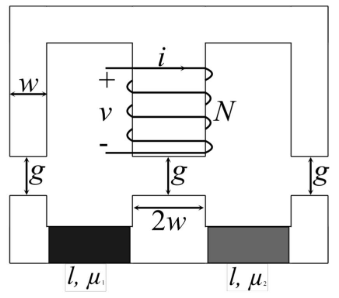
\includegraphics[width=0.4\textwidth]{figures/coreQ4.PNG}
        \caption{Bumblebee's Core}
        \label{poletradsaj}
\end{figure} \\ The width of the core is 5 cm, the gap length is 2 cm, and the depth is 3 cm. The coil's number of turns is N = 300. Neglect fringing.
\begin{enumerate}[label=(\alph*)]
    \item {What is the magnetic circuit equivalent of Bumblebee's new inductor core and coil?}
    \item {What is the inductor's new inductance?}
    \item {What is the voltage drop now across the coil in terms of the variable i?}
\end{enumerate}
\newpage %Page Three 
\noindent 
\section*{Problem 5: Energy \& Co-Energy, Force and Torque} 
The two parts of this problem are unrelated.
\begin{enumerate}[label=(\alph*)]
    \item {An electromechanical system has flux linkage given as
    $$\lambda = 5i^5e^{x^2}$$
    What is the energy, coenergy, and force of electric origin of this system?}
    \item {If the energy of an electromechanical system is given by $$W_m=i^2,$$ what is the coenergy in terms of $i$ and $\lambda$?}
\end{enumerate}

\newpage %Page Three 
\noindent 
\section*{Problem 6: EFM and EFE}  
An electromechanical system is operated over the path a $\rightarrow$ b $\rightarrow$ c, as shown in the figure below.  The system is known to be electrically linear, i.e., $\lambda=L(x)i$.

\begin{figure}[H]
        \centering
        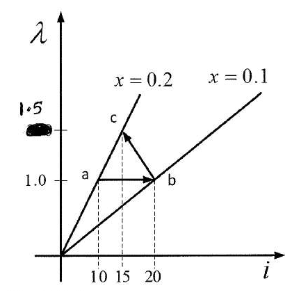
\includegraphics[width=0.4\textwidth]{figures/q6.PNG}
        \label{poletradsaj}
\end{figure}
\begin{enumerate}[label=(\alph*)]
    \item {Calculate the energy stored in the coupling field ($W_m$) at points a, b, and c.}
    \item {Calculate the EFE from a $\rightarrow$ b $\rightarrow$ c.}
    \item {Calculate the EFM from a $\rightarrow$ b $\rightarrow$ c.}
    \item{Suppose the system takes the path from a $\rightarrow$ c directly. Is the EFM from a $\rightarrow$ c equal to the EFM from a $\rightarrow$ b $\rightarrow$ c? Explain your answer. If they are NOT equal, then state the value of the EFM from a $\rightarrow$ c.}
\end{enumerate}
\newpage %Page Three 
\noindent 
\section*{Problem 7: Slippery Induction Machines (Megatron's Induction Motor)}  
\begin{enumerate}[label=(\alph*)]
    \item {Megatron starts escaping using his 3 phase, 4 pole, 400 Hz, induction motor.  If his motor has a slip of s = 0.5, what is the mechanical speed of the rotor in RPM?}
    \item {Megatron's induction motor has the following equivalent circuit. How much torque is generated, and how much real and reactive power does it draw if it operates at 100 V (line to neutral)?}
    \begin{figure}[H]
        \centering
        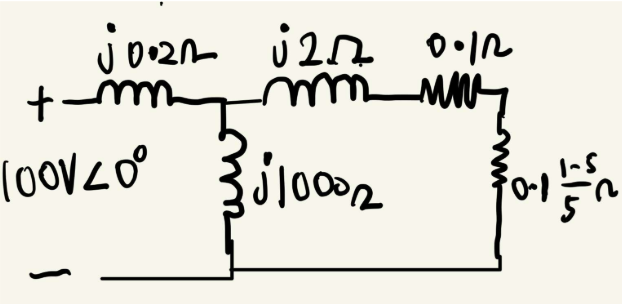
\includegraphics[width=0.6\textwidth]{figures/q7.PNG}
        \label{poletradsaj}
\end{figure}
    \item {If, under the conditions in part (b), Megatron were to perform power factor correction on his induction motor, how many VARs of capacitance would he need to obtain a unity power factor?}
\end{enumerate}
\newpage %Page Three 
\noindent 
\section*{Problem 8: Synchronous Machines (Optimus Prime's Synchronous Machine)}  
\begin{enumerate}[label=(\alph*)]
    \item {Optimus Prime is chasing Megatron down, but he is running low on power. Using the power of friendship and a 2 pole synchronous generator, the Autobots supply Optimus Prime power. If the synchronous inductance of the generator is $1/(10\pi)$ H and the field current is $5\sqrt{2}$ A, how fast must the generator spin to have an excitation voltage of 200 V?}
    \item {If the generator supplies 6 kW of power at a power factor of 0.8, then how much line current is drawn from the generator? Neglect armature resistance.}
    \item {The synchronous reactance of the generator is 2$\Omega$ and the "grid voltage" is 170 V RMS (line to neutral). What is the torque angle? (You may NOT assume the power factor is still 0.8, but you may still assume the generator is supplying 6 kW.)}
    \item{Is this synchronous machine over or underexcited? }
\end{enumerate}
\newpage %Page Three 
\noindent 
\section*{Problem 9: State Space Model} 
Optimus Prime is chasing Megatron and the distance between them is the solution to the following system of differential equations:
\begin{equation}
    V=-(x^2 + M) \nonumber
\end{equation}
\begin{equation}
    \dot{M}=4x+M \nonumber
\end{equation}
\begin{equation}
    V=\dot{x} \nonumber
\end{equation}
Using Euler's method, figure out how long it will take Optimus to reach Megatron with a time step of 100 ms, with initial conditions $x(0)=2$, $M(0)=0$.
\newpage %Page Three 
\noindent 
\section*{Problem 10: Determining Stability}
Optimus Prime has caught up to Megatron and kicks him right in his power source (OUCH!). Megatron turns around to deliver a fatal blow to Optimus, but his electromechanical system got damaged from Optimus Prime's kick! If his electromechanical system is represented by
\begin{equation}
    \frac{dx_1}{dt} = -x_1 - x_1x_2 \nonumber
\end{equation}
\begin{equation}
    \frac{dx_2}{dt} = \frac{1}{2}x_1x_2-2x_2 \nonumber
\end{equation}
\text{With initial conditions: $x_1(0) = 2, x_2(0) =0.5$}
\begin{enumerate}[label=(\alph*)]
    \item {Find all possible static equilibrium points and their eigenvalues.}
    \item {Are these points stable? Will Megatron be stable enough to deliver the fatal blow to Optimus Prime? Will Optimus Prime live? (this is all one question)}

\end{enumerate}
\end{document}
\end{document}
